\chapter{Fairness.}
\label{ch:fairness}
\only<article>{ When machine learning algorithms are applied at scale,
  it can be difficult to imagine what their effects might be. In this
  part of the book, we consider notions of fairness as seen through
  the prism of conditional independence and meritocracy. The first
  notion requires that we look deeper into directed graphical models.
  
  The problem of fairness in machine learning and
  artificial intelligence has only recently been widely
  recognised. When any algorithm is implemented at scale, no matter
  the original objective and whether it is satisfied, it has
  significant societal effects. In particular, even when considering
  the narrow objective of the algorithm, even if it improves it
  overall, it may increase inequality.
  
  In this course we will look at two aspects of fairness. The first
  has to do with disadvantaged populations that form distinct social
  classes due to a shared income stratum, race or gender. The second
  has to do with meritocratic notions of fairness.  
    
}

\section{Some examples.}


\only<article>{ Fairness is a concept that has received much attenion
  recently when applied to large-scale algorithmic decision
  making. However, the very concept of fairness is not well-defined
  and encompasses many different ideas. Some of those relate to fair
  treatment of individuals: \emph{Meritocracy} is the idea that people
  should receive rewards according to their merit. \emph{Equal
    treatment} is the related notion that similar people should be
  treated similarly under similar circumstances. Some concepts are
  related more to the treatment of different groups:
  \emph{Proportional representation} is the idea that proportions of
  different groups in society should be reflected in every facet of
  society. Finally \emph{non-discrimination} captures the notion of
  not treating people differently depending on sensitive
  characteristics.  }

\only<presentation>{
\begin{frame}
  \frametitle{Fairness}
  What is it?
  \begin{itemize}
  \item<2-> \alert{Meritocracy}.
  \item<3-> Proportionality and representation.
  \item<4-> Equal treatment.
  \item<5-> \alert{Non-discrimination}.
  \end{itemize}
\end{frame}
}

\begin{frame}
  \frametitle{Meritocracy}
  \only<article>{

    Meritocracy embodies the principle that merit should be
    rewarded. A common example are admissions to univerisities. Some
    type of summary, typically a grade obtained from high school, is
    used to represent the underlying merit of individuals.
  }
  \uncover<2->{
    \begin{example}[College admissions]
      \only<article>{ In this example, we have two students. In terms
        of grades, student $B$ is clearly better. If we can only
        accept one of them, and given no other information, it seems
        like the natural choice is student $B$.  }
      \begin{itemize}
      \item Student $A$ has a grade 4/5 from Gota Highschool.
      \item Student $B$ has a grade 5/5 from Vasa Highschool.
      \end{itemize}
    \end{example}
  }
  \only<article>{Grades, by themselves, are typically insufficient information. It might be that grades from some highschools are inflated and do not represent the quality of individuals accurately. So, let us suppose we now consider the information.}
  \uncover<3->{
    \begin{example}[Additional information]
      \only<article>{
        In particular, let us suppose that we have statistics on how well students from different high school do, depending on their high school grade.
      }
      \begin{itemize}
      \item 70\% of admitted Gota graduates with 4+ get their degree.
      \item 50\% of admitted Vasa graduates with 5 get their degree.
      \end{itemize}
      \only<article>{
        All other thing being equal, it is now more likely that student $A$ will graduate. So perhaps we should take in $A$ and not $B$.
      }
    \end{example}
  }

  \uncover<4->{We still don't know how a \alert{specific} student will
    do!}

  \only<article>{ I must emphasize that these are only
    statistics, and not necessarily predictive of the students'
    ability.  Ideally, we would like to admit the students that we
    expect to do well, given the information that we have. However,
    this information is typically not enough for us to make reliable
    predictions.  In addition, we might want to also make sure that
    everybody has a chance to obtain a good education. In order to
    achieve this, we might want to promote ethnic or gender equality
    through university admissions.  Unfortunately, there is no ideal
    solution and we must always balance the benefit of individual
    students with that of specific societal groups as well as society
    as a whole.
  }
        

\end{frame}


\only<presentation>{
  \begin{frame}
    \frametitle{Hiring decisions}
    \begin{columns}
      \begin{column}{0.5\textwidth}
        \includegraphics[height=\textheight]{../figures/cmu-headcount}
      \end{column}
      \begin{column}{0.5\textwidth}
        \includegraphics[width=\columnwidth]{../figures/amazon-hiring}
        \\
        \includegraphics[width=\columnwidth]{../figures/recruitement-automation}
      \end{column}
    \end{columns}
  \end{frame}


\begin{frame}
  \frametitle{Group fairness and proportionality}
    \includegraphics[width=\textwidth]{../figures/genomics-diversity}
    \url{https://qz.com/1367177/}
\end{frame}

}

\begin{frame}  
  \begin{block}{Solutions}
    \only<article>{These solution methods are not completely exclusive, and can be implemented simultaneously to some extent.}
    \begin{itemize}
    \item<5-> Admit \alert{everybody}? \only<article>{This suggests that everybody is admitted to at least one university, perhaps even their university of choice. However, it requires that there is enough teaching capacity for all students in the first year. Subsequently, we expect the students who were not qualified to drop out. Of course, this is unfair to the qualified students, as it drains resources that could have been used for them.}
    \item<6-> Admit \alert{randomly}? \only<article>{Completely random decisions are not considered fair, because they do not take into account any information. However, randomisation can also be used in conjunction with grades to ensure that everybody has a soht.}
    \item<7-> Use \alert{prediction} of individual academic performance? \only<article>{The more information we have, the better we can predict academic performance. A grade from high school is one indicator, but more data can be used to obtain better predictions. Of course, no prediction is perfect.}
    \item<8-> Should we take into account \alert{group membership} or other population information? \only<article>{For many reasons, students in some groups can perform differently in standardised tests, even though their innate talents may be no different than students not in the group. The classical example of this is high school teachers discouraging girls from mathematics.}
    \end{itemize}
  \end{block}
  
\end{frame}


\only<article>{
  \begin{example}[Hiring decisions.]
    As a further example, consider gender balance in hiring decisions.
    Typically, received applications are screened, so that some
    applicants undergo through an interview process. At the end, some
    of the interviewed applicants will be hired. There are two
    decision points here, with most people being cut off at the first
    point: the screening. To automate this process, Amazon worked on
    resume-screen program.~\footnote{\url{https://www.reuters.com/article/us-amazon-com-jobs-automation-insight-idUSKCN1MK08G}}
    However, this was scrapped after it was discovered that it
    predominantly favoured men. The reason is not entirely clear, but
    it was probably due to the fact that they trained the system on
    their own screening decisions, and given that the tech industry
    predominantly hires men in the first place, women were likely
    rejected in the screening phase. 
  \end{example}
}


\begin{frame}
  \frametitle{Bail decisions}

  \only<article>{ For a more detailed
    example, let us consider bail decisions in the US court
    system. When a defendant is charged, the judge has the option to
    either place them in jail pending trial, or set them free, under
    the condition that the defendant pays some amount of 'bail'. The
    amount of bail (if any) is set to deter flight or a relapse.

    This process sometimes includes the use of a software tool called
    \texttt{COMPAS}, which gives risk scores for the possibility of
    flight, recidivism or violent behaviour. These scores are taken
    into account by judges when making decisions.  In some cases, it
    appears as though automating this procedure might lead to better
    outcomes. But is that generally true?
  }

  \only<presentation>{
    \begin{columns}
      \begin{column}{0.5\textwidth}
        \centering
        \begin{tikzpicture}
          \node at (0,0) (judge) {\includegraphics[width=0.3\columnwidth]{../figures/judge}};
          \uncover<2->{
            \node at (-2,-2) (jail) {\includegraphics[width=0.3\columnwidth]{../figures/jail}};
            \draw[->] (judge) -- (jail);
          }
          \uncover<3->{
            \node at (2,-2) (bail) {\includegraphics[width=0.3\columnwidth]{../figures/bail}};
            \draw[->] (judge) -- (bail);
          }

          \uncover<4->{
            \node at (-2,-4) (trial) {\includegraphics[width=0.3\columnwidth]{../figures/trial}};
            \draw[->] (jail) -- (trial);
          }
          \uncover<5->{
            \draw[->] (bail) -- (trial);
          }
          \uncover<6->{
            \node at (2,-4) (arrest) {\includegraphics[width=0.3\columnwidth]{../figures/handcuffs}};
            \draw[->] (bail) -- (arrest);
          }
        \end{tikzpicture}
      \end{column}
      \begin{column}{0.5\textwidth}
        \centering
        \uncover<7->{
          \includegraphics[width=\textwidth]{../figures/judge-fairness}
        }
      \end{column}
    \end{columns}
  }
  

\begin{frame}
  \only<article>{Let us take the scoring of individuals.}
  \begin{figure}[H]
    \begin{columns}
      \begin{column}{0.5\textwidth}
        \centering
        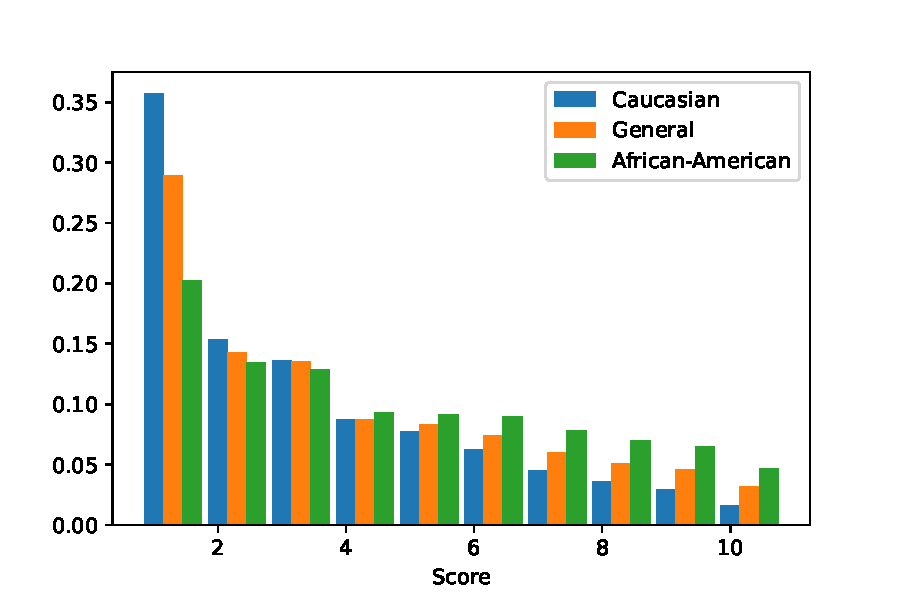
\includegraphics[width=\columnwidth]{../figures/Scores-by-race}      
        White
      \end{column}
    \end{columns}
    \label{fig:risk-bias}
    \caption{Apparent bias in risk scores towards black versus white defendants.}
  \end{figure}
\end{frame}

\begin{frame}
  \frametitle{But scores equally accurately predict recidivism\footnote{Washington Post, 2016}}
  \only<article>{On the other hand, the scores generated by the software seemed to be very predictive on whether or not defendants would re-offend, independently of their race.}
  \begin{figure}[H]
    \centering
    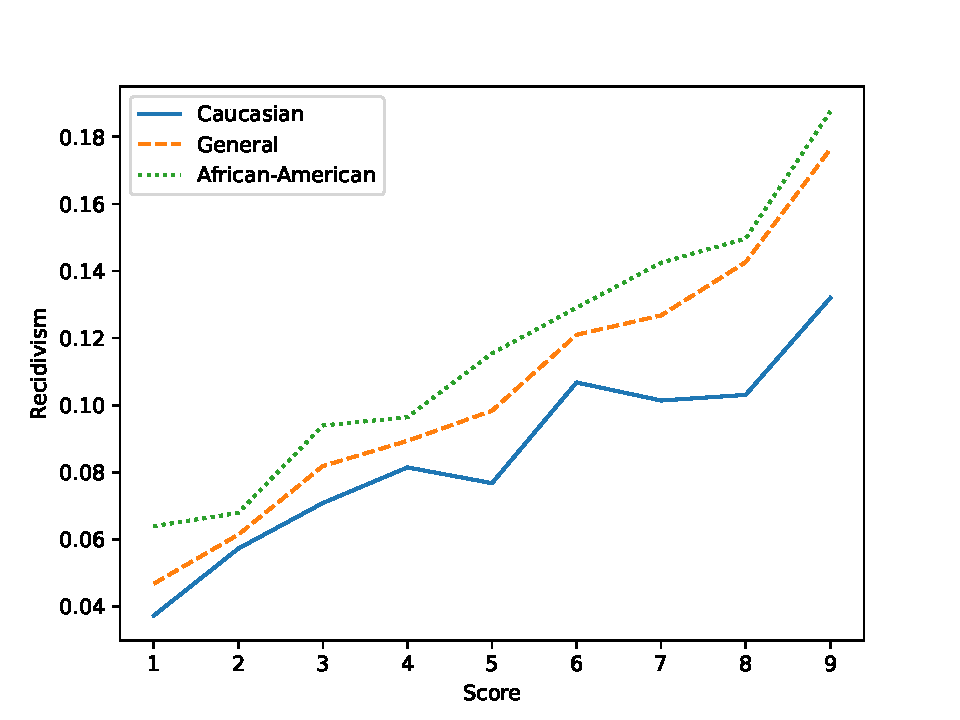
\includegraphics[width=\columnwidth]{../figures/calibration-compas}
    \caption{Recidivism rates by risk score.}
    \label{fig:imrs}
  \end{figure}
\end{frame}
\begin{frame}
  \frametitle{But non-offending blacks get higher scores}
  \only<article>{On the third hand, we see that the system seemed to give higher risk scores to non-offending blacks. So, is there a way to fix that or not?}
  \begin{figure}[H]
    \centering
    \begin{subfigure}{0.45\textwidth}
      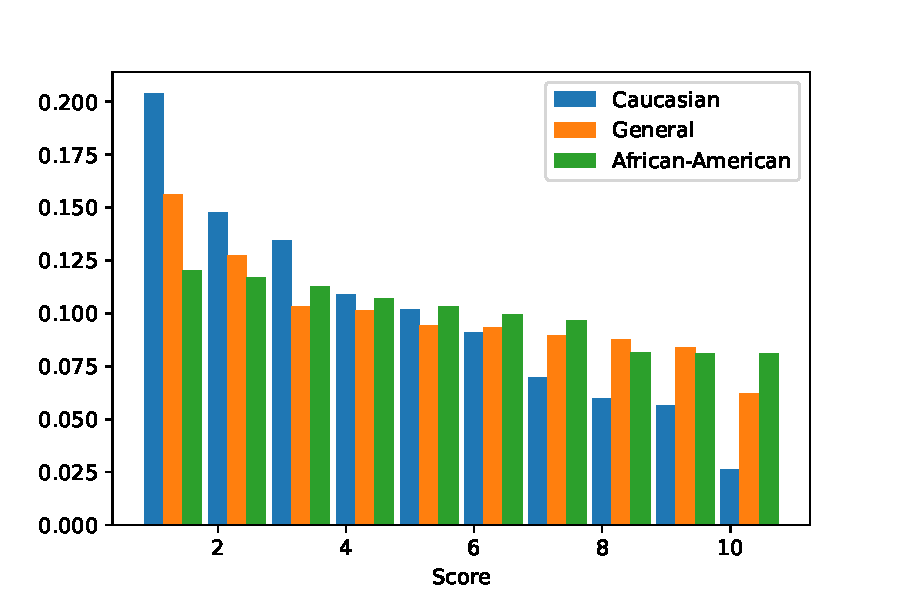
\includegraphics[width=0.95\textwidth]{../figures/balance-recidivism-compas}
    \end{subfigure}
    \begin{subfigure}{0.45\textwidth}
      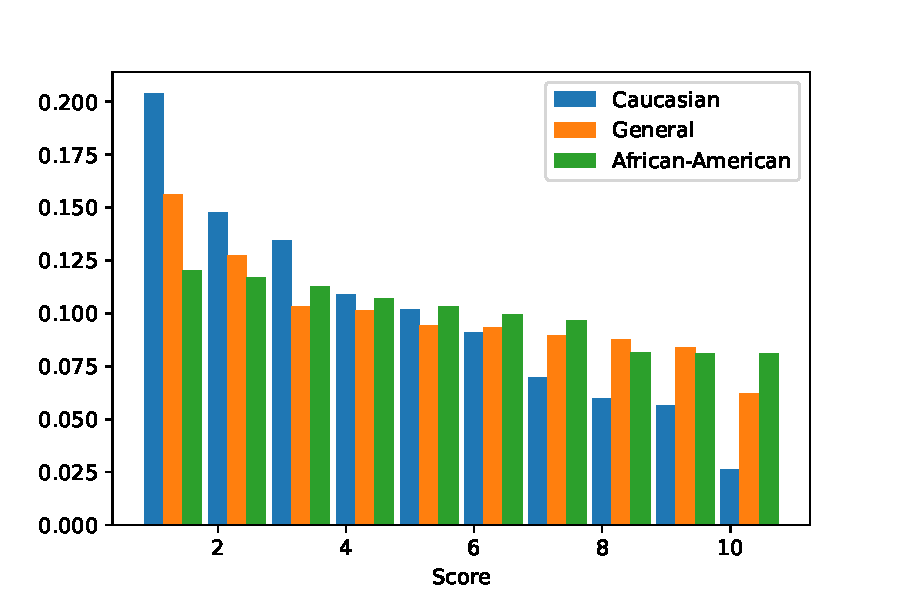
\includegraphics[width=0.95\textwidth]{../figures/balance-recidivism-compas}
    \end{subfigure}
    \caption{Score breakdown based on recidivism rates.}
    \label{fig:imrs-risk}
  \end{figure}
\end{frame}

\only<presentation>{

  \begin{frame}
    \frametitle{Graphical models and independence}
    \begin{itemize}
    \item Why is it not possible to be fair in all respects?
    \item Different notions of \alert{conditional independence}.
    \item Can only be satisfied rarely simultaneously.
    \end{itemize}
  \end{frame}

}
\only<article>{
  How can we explain this discrepancy? We can show that in fact, each one of these different measures of bias in our decision rules can be seen as a notion of conditional independence. 
}
\only<presentation>{
\chapter{Graphical models}
\label{ch:graphical-models}
\only<article>{
  Graphical models are a very useful tool for modelling the relationship between multiple variables. The simplest such models, probabilistic graphical models (otherwise known as Bayesian networks) involve directed acyclic graphs between random variables. There are two other types of probabilistic models, factor graph and undirected graphical models, which are equivalent to each other, though not to directed models.}
\begin{frame}
  \frametitle{Graphical models}
  \begin{figure}[H]
    \centering
    \begin{tikzpicture}
      \node[RV] at (2,0) (xi) {$x_3$};
      \node[RV] at (0,0) (xB) {$x_1$};
      \node[RV] at (1,1) (xD) {$x_2$};
      \draw[->] (xB) to (xD);
      \draw[->] (xD) to (xi);
      \draw[->] (xB) to (xi);
    \end{tikzpicture}
    \label{fig:bn}
    \caption{Graphical model (directed acyclic graph) for three variables.}
  \end{figure}
  \only<article>{Consider for example the model in Figure~\ref{fig:bn}. It involves three variables, $x_1, x_2, x_3$ and there are three arrows, which show how one variable depends on another. Simply put, if you think of each $x_k$ as a stochastic function, then $x_k$'s value only depends on the values of its parents, i.e. the nodes that are point to it. In this example, $x_1$ does not depend on any other variable, but the value of $x_2$ depends on the value of $x_1$. Such models are useful when we want to describe the joint probability distribution of all the variables in the collection.}

  \only<article>{The graphical model allows us to factorise the joint probability distribution of these random variables in a simplified manner. First, we define what we mean by a joint probability with respect to some probability measure $P$.}
  \begin{block}{Joint probability}
    Let $P$ is a probability measure on $(\Omega, \Sigma)$. Then let the random variable
     $\bx = (x_1, \ldots, x_n)$ so that $\bx : \Omega \to X$, $X = \prod_i X_i$. The joint probability of $\bx$ can be written in terms of the underlying probability measure $P$:
     \[
     \Pr(\bx \in A) = P(\cset{\omega \in \Omega}{\bx(\omega) \in A}).
     \]
  \end{block}
  \only<article>{
    When $X_i$ are finite, we can typically write
    \[
    \Pr(\bx = \ba) = P(\cset{\omega \in \Omega}{\bx(\omega) = \ba}),
    \]
    for the probability that $x_i = a_i$ for all $i \in [n]$.
  }
  \only<article>{Through the definition of conditional probability, we can always factorise the joint distribution of random variables as follows:}
  \begin{block}{Factorisation}
    \only<article>{
      For any subsets $B \subset [n]$ and its complement $C$ so that
      $\bx_B = (x_i)_{i \in B}$,     $\bx_C = (x_i)_{i \notin B}$
    }
    \only<1>{
      \[
      \Pr(\bx) = \Pr(\bx_B \mid \bx_C) \Pr(\bx_C)
      \only<presentation>{,\qquad B, C \subset [n]}
      \]
    }
    \uncover<2->{
      So we can write any joint distribution as
      \[
      \Pr(x_1) \Pr(x_2 \mid x_1) \Pr(x_3 \mid x_1, x_2) \cdots \Pr(x_n \mid x_1, \ldots, x_{n-1}).
      \]
    }
  \end{block}
  \only<article>{Although the above factorisation is always possible to do, sometimes our graphical model has a structure that makes the factors much simpler. In fact, the main reason for introducing graphical models is to represent dependencies between variables. For a given model, we can infer whether some variables are in fact dependent, independent, or conditionally independent.}
\end{frame}
\begin{frame}
  \frametitle{Directed graphical models and conditional independence}
  \begin{figure}[H]
    \centering
    \begin{tikzpicture}
      \node[RV] at (2,0) (xi) {$x_3$};
      \node[RV] at (0,0) (xB) {$x_1$};
      \node[RV] at (1,1) (xD) {$x_2$};
      \draw[->] (xB)--(xD);
      \draw[->] (xD)--(xi);
    \end{tikzpicture}
    \label{fig:bn}
    \caption{Graphical model for the factorisation $\Pr(x_3 \mid x_2) \Pr(x_2 \mid x_1) \Pr(x_1)$.}
  \end{figure}
  \begin{block}{Conditional independence}
    We say $x_i$ is conditionally independent of $\bx_B$ given $\bx_D$ and write $x_i \indep \bx_B \mid \bx_D $ iff
    \[
    \Pr(x_i, \bx_B \mid \bx_D)
    =
    \Pr(x_i \mid \bx_D)
    \Pr(\bx_B \mid \bx_D).
    \]
  \end{block}

  \frametitle{Directed graphical models}
  \only<article>{
    A graphical model is a convenient way to represent conditional independence between variables. There are many variants of graphical models, whose name is context dependent. Other names used in the literature are probabilistic graphical models, Bayesian networks, causal graphs, or decision diagrams. In this set of notes we focus on directed graphical models that depict dependencies between ranom variables.

    \begin{definition}[Directed graphical model] A collection of $n$ random variables $x_i : \Omega \to X_i$, and let $X \defn \prod_i X_i$, with underlying probability measure $P$ on $\Omega$.
      Let $\bx = (x_i)_{i=1}^n$ and for any subset $B \subset[n]$ let
      \begin{align}
        \bx_B &\defn (x_i)_{i \in B}\\
        \bx_{-j} &\defn (x_i)_{i \neq i}
      \end{align}
    \end{definition}
  }
  \only<article>{In a graphical model, conditional independence is represented through directed edges.}

\end{frame}

\only<article>{
  \begin{example}[Specifying a probability model]
    A graphical model does not specify the complete distribution, only
    an allowed factorisation. If we want to specify a complete
    distribution for the above graphical model of $x_1, x_2, x_3$, we
    can use the following notation:
    \begin{align}
      \label{eq:factored-model}
      x_1 &\sim f\\
      x_2 \mid x_1 = a &\sim g(a)\\
      x_3 \mid x_2 = b &\sim h(b),
    \end{align}
    where $f, g, h$ are three different distributions, with $g$ and $h$ being specified through a single parameter.
  \end{example}
}
\begin{frame}
  \begin{example}[Smoking and lung cancer]
    \begin{figure}[H]
      \centering
      \begin{tikzpicture}
        \node[RV] at (0,0) (x1) {$S$};
        \node[RV] at (1,1) (x2) {$C$};
        \node[RV] at (2,0) (x3) {$A$};
        \draw[->] (x1)--(x2);
        \draw[->] (x3)--(x2);
      \end{tikzpicture}
      \caption{Smoking and lung cancer graphical model, where $S$: Smoking, $C$: cancer, $A$: asbestos exposure.}
    \end{figure}
    \only<article>{
      It has been found by~\citet{lee2001relation} that lung  incidence not only increases with both asbestos exposure and smoking. This is in agreement with the graphical model shown. The study actually found that there is an amplification effect, whereby smoking and asbestos exposure increases cancer risk by 28 times compared to non-smokers. This implies that the risk is not simply additive. The graphical model only tells us that there is a dependency, and does not describe the nature of this dependency precisely.}
  \end{example}
  \begin{block}{Explaining away}
    Even though $S, A$ are independent, they become dependent once you know $C$. \only<article>{For example, let us say we know that you have cancer and that our model says that it's very unlikely to have cancer unless you either smoke or are exposed to asbestos. When we also learn that you do not have asbestos exposure, smoking becomes more likely. In either words, if cancer is caused by either smoking or asbestos, and we rule out asbestos, the only remaining explanation is smoking. This is what is generally called \alert{explaining away.}}
  \end{block}
\end{frame}

\begin{frame}
  \begin{example}[Time of arrival at work]
    \begin{figure}[H]
      \centering
      \begin{tikzpicture}
        \node[RV] at (0,0) (x1) {$x_1$};
        \node[RV] at (1,1) (x2) {$T$};
        \node[RV] at (2,0) (x3) {$x_2$};
        \draw[->] (x2)--(x3);
        \draw[->] (x2)--(x1);
      \end{tikzpicture}
      \caption{Time of arrival at work graphical model where $T$ is a traffic jam and $x_1$ is the time John arrives at the office and $x_2$ is the time Jane arrives at the office.}
    \end{figure}
    \only<article>{
      In this model, the arrival times of John and Jane may seem correlated. However, there is a common cause: The existence of a traffic jam. Whenever there is a traffic jam, both John and Jane are usually late. Whenever there is not a traffic jam, they are both mostly on time.
    }
  \end{example}
  \begin{block}{Conditional independence}
    Even though $x_1, x_2$ are correlated, they become independent once you know $T$.
  \end{block}
\end{frame}

\begin{frame}
  \begin{example}[Treatment effects]
    \begin{figure}[H]
      \centering
      \begin{tikzpicture}
        \node[RV] at (0,0) (x) {$x$};
        \node[RV] at (1,1) (y) {$y$};
        \node[RV] at (2,0) (a) {$a$};
        \draw[->] (x)--(y);
        \draw[->] (x)--(a);
        \draw[->] (a)--(y);
      \end{tikzpicture}
      \caption{Kidney treatment model, where $x$: severity, $y$: result, $a$: treatment applied}
    \end{figure}
    \begin{table}[H]
      \begin{tabular}{l|r|r}
        & Treatment A  & Treatment B\\
        \hline
        Small stones & 87  & 270\\
        Large stones  & 263 &  80
      \end{tabular}
      \begin{tabular}{l|r|r}
        Severity & Treatment A  & Treatment B\\
        \hline
        Small stones ) & 93\%  & 87\%\\
        Large stones  & 73\% &  69\%\\
        \hline
        Average & 78\% & 83\%
      \end{tabular}
    \end{table}
    \only<article>{
       A curious example is that of applying one of two treatments for kidneys. In the data, it is clear that one treatment is best for both large and small stones. However, when the data is aggregated it appears as though treatment B is best. This is because treatment A is chosen much more frequently when the stones are large, and that's when both treatments perform worse. This apparent discrepancy is called \emph{Simpson's paradox}\index{Simpson's paradox}}
  \end{example}
\end{frame}


\begin{frame}
  \begin{example}[School admission]
    \begin{figure}[H]
      \centering
      \begin{subfigure}{0.45\textwidth}
        \begin{tikzpicture}
          \node[RV] at (0,0) (z) {$z$};
          \node[RV] at (1,1) (s) {$s$};
          \node[RV] at (2,0) (a) {$a$};
          \draw[->] (z)--(s);
          \draw[->] (z)--(s);
          \draw[->] (s)--(a);
        \end{tikzpicture}
      \end{subfigure}
      \begin{subfigure}{0.45\textwidth}
        \begin{tikzpicture}
          \node[RV] at (0,0) (z) {$z$};
          \node[RV] at (1,1) (s) {$s$};
          \node[RV] at (2,0) (a) {$a$};
          \draw[->] (z)--(s);
          \draw[->] (z)--(s);
          \draw[->] (s)--(a);
          \draw[->] (z)--(a);
        \end{tikzpicture}
      \end{subfigure}
      \caption{School admission graphical model, where $z$: gender, $s$: school applied to, $a$: whether you were admitted. }
    \end{figure}
    \begin{table}[H]
      \begin{tabular}{l|r|r}
        School & Male  & Female\\
        \hline
        A & 62\% & 82\%\\
        B & 63\% & 68\%\\
        C & 37\% & 34\%\\
        D & 33\% & 35\%\\
        E & 28\% & 24\%\\
        F &  6\% &  7\%\\
        \hline
        \emph{Average} & \emph{45\%} & \emph{38\%}
      \end{tabular}
    \end{table}
    \only<article>{In this example, it appears as though female candidates have a lower acceptance rate than males. However what is missing is the fact that many more males are applying to easier schools. Thus, it is possible that the data is explainable by the fact that admission only reflects the difficulty of each school, and the overall gender imbalance is due to the choices made by the applicants. However, an alternative model is that the admissions process also explicitly takes gender into account. However, both of these models may be inadequate, as we do not have data about each individual applicant, such as their grades. We shall discuss this issue further when we talk about causality, confounding variables and counterfactuals.}
  \end{example}
\end{frame}


\input{graphical-models-exercises.tex}



\begin{frame}
  \begin{alertblock}{Deciding conditional independence}
    There is an algorithm for deciding conditional independence of any two variables in a graphical model.
    \only<article>{However, this is beyond the scope of these notes. Here, we shall just use these models as a way to encode dependencies that we assume exist.}
  \end{alertblock}

\end{frame}

\section{Inference and prediction in graphical models}
\begin{frame}
\frametitle{Inference and prediction in graphical models}
 \begin{figure}[H]
     \centering
     \begin{tikzpicture}
       \node[RV, hidden] at (0,0) (param) {$\param$};
       \node[RV] at (-1,1) (data1) {$x_1$};
       \node at (0,1) (data2) {$\cdots$};
       \node[RV] at (1,1) (data3) {$ x_t$};
       \draw[->] (param)--(data1);
       \draw[->] (param)--(data3);
       \node<2->[RV] at (2,1) (new_data) {$x_{t+1}$};
       \draw<2->[->] (param)--(new_data);
     \end{tikzpicture}
     \caption{Inference and prediction in a graphical model}. 
   \end{figure}
\only<article>{In this example, $x_1, \ldots, x_t$ are all i.i.d, drawn from the distribution $P_\param(x_t) = \Pr(x_t \mid \param)$.}
  \only<1>{
    \begin{block}{Inference of latent variables}\index{inference}
      \[
      \Pr(\param \mid x_1, \ldots, x_t)
      \]
      \only<article>{Inference in graphical models typically refers to the problem of estimating the distribution of some \emph{hiddeen} or \emph{latent} variable from data. These variables are generally thought of as two types:}
      \begin{itemize}
      \item Model parameters. \only<article>{These generally do not change over time. One example is estimating the mean of a Gaussian distribution from data.}
      \item System states. \only<article>{These typically are time-indexed. We will see further examples of such variables when we discuss latent variable models. On example is inferring location from GPS measurements.} 
      \end{itemize}
    \end{block}
  }
  \only<2>{
    \begin{block}{Prediction}\index{prediction}
      \[
      \Pr(x_{t+1} \mid x_1, \ldots, x_t)
      =
      \int_\Param \Pr(x_{t+1} \mid \param) \dd \Pr(\param \mid x_1, \ldots, x_t)
      \]
      \only<article>{Prediction is a type of inference, but differs in that the variable whose distribution we wish to estimate is only temporarily not observed: we can actually obtain its value in the future. Thus, a prediction is always testable!}
      \only<presentation>{
        Predictions are \alert{testable.}
      }
    \end{block}
  }
\end{frame}

\begin{frame}
\frametitle{Coin tossing, revisited}
\begin{example}{The Beta-Bernoulli prior}
  \begin{figure}[H]
    \centering
    \begin{tikzpicture}
      \node[RV] at (0,0) (bel) {$\bel$}; \node[RV, hidden] at (1,0)
      (param) {$\param$}; \node[RV] at (2,0) (data) {$x$}; \draw[->]
      (bel)--(param); \draw[->] (param)--(data);
    \end{tikzpicture}
    \caption{Graphical model for a Beta-Bernoulli prior}
  \end{figure}
  \begin{align}
    \param &\sim \BetaDist(\bel_1, \bel_2), && \textrm{i.e.  $\bel$ are Beta distribution parameters}\\
    x \mid \param &\sim \Bernoulli(\param), && \textrm{i.e. $P_\param(x)$ is a Bernoulli}
  \end{align}
  \only<article>{In this example, it is obvious why we use the notation above for describing hierarchical models.\index{hierarchical Bayesian model} We simply state what is the distribution on one variable conditioned on the other variables. Here, $\bel$ is fixed, and it is something we can choose arbitrarily. The data $x$ is observed, while the parameter $\param$ remains \emindex{latent}. Using Bayes theorem, we can derive the distribution for $\bel(\theta \mid x)$. In this particular case, we elide referring to a sample $x_1. \ldots, x_t$ as they are all i.i.d.}
\end{example}
\end{frame}

\begin{frame}
  \begin{example}{The $n$-meteorologists problem (continuation of Exercise~\ref{ex:meteorologists})}\index{$n$-meteorologists}
    \only<presentation>{
      \begin{itemize}
      \item Meteorological models $\CM = \set{\model_1, \ldots, \model_n}$
      \item Rain predictions at time $t$: $p_{t,\model} \defn  P_{\model}(x_t = \textrm{rain})$.
      \item Prior probability $\bel(\model) = 1/n$ for each model.
      \item Decision $a$, resulting in utility $\util(a, x_{t+1})$
      \end{itemize}
    }
    \begin{figure}[H]
      \centering
      \begin{tikzpicture}
        \node[RV] at (0,-1) (bel) {$\bel$};
        \node[RV, hidden] at (0,0) (param) {$\model$};
        \node[RV] at (-1,1) (data1) {$x_1$};
        \node at (0,1) (data2) {$\cdots$};eu
        \node[RV] at (1,1) (data3) {$ x_t$};
        \draw[->] (param)--(data1);
        \draw[->] (param)--(data3);
        \node[RV] at (2,1) (new_data) {$x_{t+1}$};
        \draw[->] (param)--(new_data);
        \draw[->] (bel)--(param);
        \node[select] at (2,-1) (act) {$a$};
        \node[utility] at (4,-1) (util) {$\util$};
        \draw[->] (act)--(util);
        \draw[->] (new_data)--(util);
        \draw[->] (data3)--(new_data);
        \draw[->] (data1) to [bend left] (new_data);
        \draw[->] (data1) to [bend right] (data3);
      \end{tikzpicture}
     \caption{Inference, prediction and decisions in a graphical model.}
   \end{figure}
   \only<article>{In this problem, we allow each model's predictions to have arbitrary dependences with the past i.e.
     \[
     P_\model(x_{t+1} \mid x_t, x_{t-1}, \ldots, x_1).
     \]
     For inference, the details of how each model works are not important: just the probability of the next observation given the previous ones.
   }
  \end{example}


\end{frame}


\section{Testing conditional independence}
\begin{frame}
  \frametitle{Measuring independence}
  \only<article>{The simplest way to measure independence is by looking at whether or not the distribution of the possibly dependent variable changes when we change the value of the other variables. }

  \begin{theorem}
    If $x_i \indep \bx_B  \mid \bx_D$ then
    \[
    \Pr(x_i \mid \bx_B, \bx_D)
    =
    \Pr(x_i \mid \bx_D)
    \]
  \end{theorem}
  \uncover<2->{
    This implies
    \[
    \Pr(x_i \mid \bx_B = b, \bx_D)
    =
    \Pr(x_i \mid \bx_B = b', \bx_D)
    \]
    so we can measure independence by seeing how the distribution of $x_i$ changes when we vary $\bx_B$, keeping $\bx_D$ fixed.
  }
    \only<article>{For any given model, there is either a dependence or there is not. However, sometimes we might be able to tolerate some amount of dependence. Thus, we can simply measure the deviation from independence through a metric or divergence on distributions.}
  \begin{example}
    \[
    \|\Pr(a \mid y, z) - \Pr(a \mid y)\|_1
    \]
    which for discrete $a,y,z$ is:
    \[
    \max_{i,j} \|\Pr(a \mid y = i, z = j) - \Pr(a \mid y= i)\|_1
    =
    \max_{i,j} \|\sum_k \Pr(a = k \mid y = i, z = j) - \Pr(a =k \mid y= i)\|_1.
    \]
    See also \url{src/fairness/ci_test.py}
  \end{example}
\end{frame}


\begin{frame}
\begin{example}{An alternative model for coin-tossing}
  This is an elaboration of Example~\ref{ex:bayesian-compound-hypothesis-test} for hypothesis testing.
  \begin{figure}[H]
    \centering
    \begin{tikzpicture}
      \node[RV] at (-1,0) (hbel) {$\hyperparam$};
      \node[RV] at (1,1) (bel) {$\bel$};
      \node[RV, hidden] at (0,0) (model) {$\model$};
      \node[RV, hidden] at (1,0) (param) {$\param$};
      \node[RV] at (2,0) (data) {$x$};
      \draw[->] (hbel)--(model);
      \draw[->] (bel)--(param);
      \draw[->] (model)--(param);
      \draw[->] (param)--(data);
    \end{tikzpicture}
    \caption{Graphical model for a hierarchical prior}
  \end{figure}
  \begin{itemize}
  \item $\model_1$: A Beta-Bernoulli model with $\BetaDist(\bel_1, \bel_2)$
  \item $\model_0$: The coin is fair.
  \end{itemize}
  \begin{align}
    \param \mid \model = \model_0 &\sim \Singular(0.5), && \textrm{i.e. $\param$ is always 0.5}\\
    \param \mid \model = \model_1 &\sim \BetaDist(\bel_1, \bel_2), && \textrm{i.e. $\param$ has a Beta distribution}\\
    x \mid \param &\sim \Bernoulli(\param), && \textrm{i.e. $P_\param(x)$ is Bernoulli}
  \end{align}
  Here the posterior over the two models is simply
  \[
  \hyperparam(\model_0 \mid x) = \frac{P_{0.5}(x) \hyperparam(\model_0)}{P_{0.5}(x) \hyperparam(\model_0) + \Pr_{\model_1}(x) \hyperparam(\model_1)},
  \qquad
  \Pr_{\model_1(x)} = \int_0^1 P_\param(x) \dd \bel(\param).
  \]
\end{example}

\end{frame}

\begin{frame}
  \frametitle{Bayesian testing of independence}
  \only<article>{
    For a given distributional model $P_\param$, conditional independence either holds or does not. Consider the set of model parameters $\Param_0$ where, for each parameter $\param \in \Param_0$, we have a conditional independence condition, while $\Param_1$ may corresponds to models where there may not be independence. To make this more concrete, let's give an example.}

    \begin{figure}[H]
      \centering
      \begin{subfigure}[b]{0.45\textwidth}
        \begin{tikzpicture}
          \node[RV] at (0,0) (x1) {$x_1$};
          \node[RV] at (1,1) (x2) {$x_2$};
          \node[RV] at (2,0) (x3) {$x_3$};
          \draw[->] (x1)--(x2);
          \draw[->] (x2)--(x3);
        \end{tikzpicture}
        \caption{$\Param_0$ assumes independence}
      \end{subfigure}
     \begin{subfigure}[b]{0.45\textwidth}
     \begin{tikzpicture}
        \node[RV] at (0,0) (x1) {$x_1$};
        \node[RV] at (1,1) (x2) {$x_2$};
        \node[RV] at (2,0) (x3) {$x_3$};
        \draw[->] (x1)--(x2);
        \draw[->] (x2)--(x3);
        \draw[alert,->] (x1)--(x3);
      \end{tikzpicture}
      \caption{$\Param_1$ does \alert{not} assume independence}
    \end{subfigure}
    \only<article>{\caption{The two alternative models}}
    \end{figure}
  \begin{example}
    \only<1>{
    Assume data $D = \cset{x^t_1, x^t_2, x^t_3}{t = 1, \ldots, T}$ with $x_i^t \in \set{0,1}$.
    \only<article>{First consider model $\Param_0$ where the following conditional independence holds
    \[
    P_\param(x_3 \mid x_2, x_1) = P_\param(x_2 \mid x_1), \qquad \forall \param \in \Param_0.
    \]
    In the alternative model $\Param_1$ there is no
      independence assumption. So the likelihood for either a model in either set is}
    \begin{align}
    P_\param(D) &= \prod_t P_\param(x^t_3 \mid x^t_2) P_\param(x^t_2 \mid x^t_1) P_\param(x^t_1), \qquad \param \in \Param_0\\
    P_\param(D) &= \prod_t P_\param(x^t_3 \mid x^t_2, \alert{x_1^t}) P_\param(x^t_2 \mid x^t_1) P_\param(x^t_1), \qquad \param \in \Param_1
    \end{align}
  }
  \only<2>{
    \only<article>{The parameters for this example can be defined as follows}
    \begin{align}
      \param_1 &\defn P_\param(x^t_1 = 1) \tag{$\model_0,\model_1$}\\
      \param_{2|1}^{i} &\defn P_\param(x^t_2 = 1 \mid x^t_1 = i) \tag{$\model_0, \model_1$}\\
      \param_{3|2}^{j} &\defn P_\param(x^t_3 = 1 \mid x^t_2 = j) \tag{$\model_0$}\\
      \param_{3|2,1}^{i,j} &\defn P_\param(x^t_3 = 1\mid x^t_2=j, x_1^t=i)\tag{$\model_1$}
    \end{align}
    \only<article>{
      We model each one of these parameters with a separate Beta-Bernoulli distribution.
    }
  }
  \end{example}

\end{frame}



\section{Hierarchical Bayesian models}
\begin{frame}
\only<article>{Given some data $D$, the Bayesian approach would involve specifying a hierarchical prior\index{hierarchical Bayesian model} $\bel$ so that $\hyperparam(\model_1) = 1 - \hyperparam(\model_0)$ specifies a probability on the two model structures, while for the $i$-th model we define a prior $\bel_i(\param)$ over $\Param_i$, so that we obtain the following hierarchical model
  }
  \begin{figure}[H]
    \centering
    \begin{tikzpicture}
      \node[RV, hidden] at (0,0) (model) {$\model$};
      \node[RV, hidden] at (1,0) (param) {$\param$};
      \node[RV] at (2,0) (data) {$D$};
      \draw[->] (model)--(param);
      \draw[->] (param)--(data);
    \end{tikzpicture}
        \caption{Hierarchical model.}
    \label{fig:hierarchical-model}
  \end{figure}
\only<article>{Here the specific model $\model$ is unobserved, as well as its parameters $\param$. Only the data $D$ is observed. Our prior distribution is omitted from the graph.}
\only<1>{
\begin{align}
  \model_i &\sim \hyperparam\\
  \param \mid \model = \model_i &\sim \bel_i
\end{align}
}
\only<1->{
  \begin{block}{Marginal likelihood}
    \only<article>{This gives the the following marginal likelihood for the combined models and each of the models respectively.}
    \begin{align}
      \Pr_\hyperparam(D) &= \hyperparam(\model_0) \Pr_{\model_0}(D)  + \hyperparam(\model_1) \Pr_{\model_1}(D)\\
      \Pr_{\model_i}(D) &= \int_{\Param_{i}} P_{\param}(D) \dd \bel_i(\param).
    \end{align}
  \end{block}
}
\only<2->{
  \begin{block}{Model posterior}
    \begin{equation}
      \hyperparam(\model \mid D) = 
      \frac{\Pr_\model(D) \hyperparam(\model)}
      {\sum_{i} \Pr_{\model_i} (D) \hyperparam(\model_i)}
    \end{equation}
  \end{block}
}
\end{frame}

\begin{frame}
  \frametitle{Calculating the marginal likelihood}
  \only<article>{Generally speaking, calculating the marginal likelihood for a model with an uncountable parameter set is hard. However, conjugate models admit closed form solutions and efficient calculations. Firstly, let's rewrite the marginal likelihood in terms of an integral Monte-Carlo approximation.}
  \begin{block}{Monte-Carlo approximation}
    \begin{align}
      \label{eq:mc-marginal-likelihood}
      \int_\Param P_\param(D) \dd \bel(\param)
      &\approx
        \frac{1}{N} \sum_{n=1}^N P_{\param_n}(D)  + O(1/\sqrt{N}), & \param_n &\sim \bel
    \end{align}
  \end{block}
  \only<article>{Even though this approximation is reasonable at first glance, the problem is that the leading constant of the error scales approximately proportionally to the maximum likelihood $\max_\param P_\param(D)$. This is a consequence of Hoeffding's inequality~\eqref{eq:Hoeffding}. Thus, the more data we have the more samples we need to get a good approximation with this simple Monte Carlo approach. For that reason, one typically uses a sample from a proposal distribution $\psi$ which is different from $\bel$. Then it holds}
  \begin{block}{Importance sampling}
    \only<article>{For any two measures $\bel, \psi$ on $\Param$, we can write:}
    \index{importance sampling}
    \begin{align}
      \label{eq:importance-sampling}
      \int_\Param P_\param(D) \dd \bel(\param)
      &
        \only<2>{
        =
        \int_\Param P_\param(D) \frac{\dd \psi(\param)}{\dd \psi(\param)} \dd \bel(\param)
        }
        \only<3>{
        =
        \int_\Param P_\param(D) \frac{\dd \bel(\param)}{\dd \psi(\param)} \dd \psi(\param)
        }
        \uncover<4>{
        \approx
        \sum_{n=1}^N P_\param(D) \frac{\dd \bel(\param_n)}{\dd \psi(\param_n)}, & \param_n \sim \psi
        }
    \end{align}
    \only<article>{This allows us to estimate the marginal likelihood with respect to a belief $\bel$ by sampling from an alternative belief $\psi$.}
  \end{block}
\end{frame}

\begin{frame}
  \begin{block}{Sequential updating of the marginal likelihood}
    \begin{align}
      \label{eq:sequential-likelihood}
      \Pr_\bel(D)
      \uncover<2->{
      &= \Pr_\bel(x_1, \ldots, x_T) 
        }
      \uncover<3->{
      \\
      & = \Pr_\bel(x_2, \ldots, x_T \mid x_1) \Pr_\bel(x_1)
        }
      \uncover<4->{
      \\
      & = \alert{\prod_{t=1}^T \Pr_\bel(x_t \mid x_1, \ldots, x_{t-1})}
        }
        \uncover<5->{
      \\
      & = \prod_{t=1}^T \int_\Param P_{\param_n}(x_t) \dd \underbrace{\bel(\param \mid x_1, \ldots, x_{t-1})}_{\textrm{posterior at time $t$}}
        }
    \end{align}
    \only<article>{The nice thing about this break down is that for a simple model such as Beta-Bernoulli, the individual datapoint marginal likelihoods are easy to compute}
  \end{block}
  \begin{example}[Beta-Bernoulli]
    \only<article>{The marginal predictive distribution for a Beta-Bernoulli prior is}
    \index{hierarchical Bayesian model, Beta-Bernoulli}
    \[\Pr_\bel(x_t = 1 \mid x_1, \ldots, x_{t-1}) = \frac{\alpha_t}{\alpha_t + \beta_t},
    \]
    with
    $\alpha_t = \alpha_0 + \sum_{n=1}^{t-1} x_n, \quad \beta_t = \beta_0 + \sum_{n=1}^{t-1} (1 - x_n)$
  \end{example}
\end{frame}
\begin{frame}
  \frametitle{Further reading}
  \begin{block}{Python sources}
    \begin{itemize}
    \item A simple python measure of conditional independence \url{src/fairness/ci_test.py}
    \item A simple test for discrete Bayesian network \url{src/fairness/DirichletTest.py}
    \item Using the PyMC package \url{https://docs.pymc.io/notebooks/Bayes_factor.html} 
    \end{itemize}
  \end{block}
\end{frame}

%%% Local Variables:
%%% mode: latex
%%% TeX-engine: xetex
%%% TeX-master: "notes"
%%% End:

}




%%% Local Variables:
%%% mode: latex
%%% TeX-engine: xetex
%%% TeX-master: "notes"
%%% End:
